%!TEX root = ../thesis.tex
\chapter{Estimating Defect Probabilities} \label{chap:estimating-dp}

\section*{}

In order to estimate the defect probability of each software component we developed a data mining application, agnostic to the project's language. 
It automatically extracts data from the current state and about older defects from a \emph{Git} repository, creates a model and predicts the probability. The project is written in Javascript (Node.js) and Python 3 and heavily uses \emph{node-git}
and \emph{scikit-learn}.

In this chapter, we will explain the concept behind it, approach the process used in each of the steps and will explain how to install and use this application.

\section{Concept}

Some patterns are easily recognizable when trying to identify faulty components on a software project and this information could be helpful for software such as Barinel. 

We might say, for example that having a high number of recent changes or having been changed by a given junior developer new to the project probably increases the chances of a file having an error, due to past experiences. So, deep down we are just assuming that the knowledge of the meta-data of old faulty components may allow us to predict which components are more probable to be faulty, now.

Based on that assumption, the application, for a given repository state, extracts meta-data knowledge from past commits with faulty components, the parent commits of a fix. For each of these commits, all of components are analyzed and labeled as faulty or clean, if it was or not changed on the fix, respectively.
%
% CHOURIÇO:
%
%\begin{figure}[H]
%  \begin{center}
%    \leavevmode
%    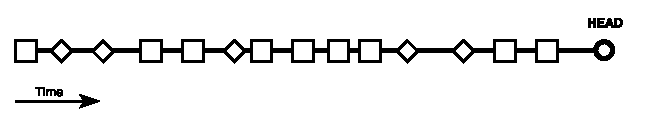
\includegraphics[width=0.7\textwidth]{commits.pdf}
%    \caption{Example representation of commits history, with fix commits illustrated in a diamond shape}
%    \label{fig:commits}
%  \end{center}
%\end{figure}

Since the application should be able to predict the defect probability for any given software project that uses \emph{Git}, static analysis is not used. 
The only information that is used is information directly related to the file changes, authors, number of lines or bytes.

Along with the extraction of the meta-data information from the past faulty states, it must also extract the meta-data of the given repository state. The data from the first extraction must be used to create a machine learning model, that should be able to predict the defect probability of each component presents in the current state of the project.
%
\begin{figure}[ht]
  \begin{center}
    \leavevmode
    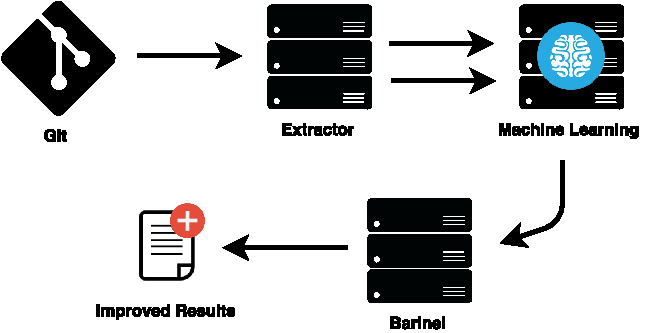
\includegraphics[width=0.7\textwidth]{concept.pdf}
    \caption{Representation of data flow}
    \label{fig:concept}
  \end{center}
\end{figure}

This concept differs from Data-Augmented Software Diagnosis (Subsection \label{subsec:elmishali}) by being language agnostic, requiring a different set of features mostly focused on number of changes, categorized by type and authors, and weighted according to size and date. It also differs by not requiring that the project uses a bug tracking software and also, as explained in the following section. 

\section{Install}

The application relies on \emph{Redis}, \emph{Git}, \emph{Node.js} and \emph{Python 3} and requires some dependencies such as \emph{SciPy}, \emph{scikit-learn}, \emph{numpy}.

\begin{lstlisting}
  $ git clone --depth 1 https://github.com/atduarte/master-thesis.git
  $ cd master-thesis/app
  $ npm install --prod
\end{lstlisting}

\section{Usage}

Having all the required dependencies installed, the usage is very straight-forward.
In order to automatically execute all the steps (extraction, data preparation, modeling and prediction) the following command should be used
by replacing "\code{{project-name}}" and "\code{{repository-path}}" respectively with
the chosen project name and the path to the folder containing the repository we want to analyze:

\begin{lstlisting}
  $ node index.js all {project-name} {repository-path}
\end{lstlisting}

It is possible to specify a different classification label (e.g. "\code{--classification-label=_mostChanged}", default is "\code{_mostChanged25}"), 
a different number of estimators used when modeling (e.g. "\code{--estimators=100}", default is 5) or even
to define the level of logging by appending, for example, "\code{--log-level=verbose}". The existing levels available, from higher to lower priority, are
"\code{error}", "\code{warn}", "\code{info}", "\code{verbose}" and "\code{silly}". The default log level is "\code{info}".

\begin{lstlisting}[style=npmlog]
  ?$  node index.js all math ../../tests/Math001?
  @info@ !extract/extract! Raw Extraction started
  @info@ !extract/extract! 499 fix commits found
  @info@ !prepareJson/prepare! JSON Preparation started
  @info@ !prepareJson/prepare! Will prepare 639 files
  @info@ !results/prepare! CSV Preparation started
  @info@ !results/prepare! Got 552 files
  @info@ !results/prepare! Got 203 columns
  @info@ !results/ml! Modeling
\end{lstlisting}

Some extra configurations are also available by creating a project configuration file, in the folder "\code{project-config/}", with the same name as the \code{project-name} plus ".js".
It allows to change the \emph{regex} used to identify the fix commits, to define a file filter and to define an email normalizer, in order to improve the quality of the extracted data .

\begin{lstlisting}[language=Javascript]
  'use strict';

  module.exports = {
      fileFilter: (filename) => {
          filename = filename.toLowerCase();

          return filename.endsWith('.java') // Is Java
              && !filename.startsWith('src/test'); // Aren't tests
      },
  };
\end{lstlisting}

Before terminating, the application will create a file ("\code{prediction.e500._mostChanged25.csv}", by default) in the repository folder containing the predicted defect probability for each source code file.

\begin{lstlisting}
  ...
  src/main/java/org/joda/time/Chronology.java,0.0
  src/main/java/org/joda/time/DateMidnight.java,0.21
  src/main/java/org/joda/time/DateTime.java,0.484
  src/main/java/org/joda/time/DateTimeComparator.java,0.0
  src/main/java/org/joda/time/DateTimeConstants.java,0.0
  src/main/java/org/joda/time/DateTimeField.java,0.006
  src/main/java/org/joda/time/DateTimeFieldType.java,0.002
  src/main/java/org/joda/time/DateTimeUtils.java,0.966
  src/main/java/org/joda/time/DateTimeZone.java,0.414
  src/main/java/org/joda/time/Days.java,0.0
  ...
\end{lstlisting}

In order to be able to execute only some step of the process, there is the possibility of executing only one operation. The available commands are:
%
\begin{itemize}
\item "\code{raw}" - Extracts data from \emph{Git} and saves it to "\code{out/{project-name}/raw}"
\item "\code{json}" - Processes the raw data and converts it to a new JSON structure. Results are saved to "\code{out/{project-name}/json}"
\item "\code{results}" - Creates the CSV files for training and prediction data, based on the JSON files, creates the model and predicts the defect probability.
Final result is saved at "\code{{repository-path}/prediction.csv}".
\end{itemize}

\section{Process}

As stated before the process is divided in extraction, data preparation, modeling and prediction steps. We will now dive deep into each.

\subsection{Extraction}

The first objective is to get the list of commits to analyze: the HEAD commit and all the fix commits that preceded it. 
So, first, the \emph{HEAD} commit is identified. The application then walks recursively through each parent commit or commits and,
if it is message matches the following regex and it is not a merge, adds it to the list of commits to analyze.

\begin{lstlisting}
(\b|)fix(|\b|ed|ing)|bug( | \#|\-|)[0-9]+
\end{lstlisting}

Having this list, it analyzes each commit individually, ignoring the ones that were already extracted or that have no changed files after filtering according to configuration.
First the information directly related to the commit and its tree is extracted:
%
\begin{itemize}
\item id - Id
\item message - Message
\item date - Date
\item author - Author
\item components - List of components
\end{itemize}

Then, the application walks through the changes history of each component, following name changes and extracting this info for each commit:
%
\begin{itemize}
\item id - Id
\item date - Date
\item author - Author
\item parentCount - Parent count
\item isFix - Is it a fix?
\item filename - Filename
\item lines - Number of lines
\item byteSize - Size of file in bytes
\item linesAdded - Number of lines added
\item linesRemoved - Number of lines removed
\end{itemize}

This data is then saved to a file named according to the commit id, in the "\code{raw}" folder (e.g "\code{out/math/raw/17d6f2163db436518f953166c1e9d495232f90b6}").

\begin{lstlisting}
{
  "id": "0b1b9a9dc86da871ce5e7839b1b2df13c99dd9f8",
  "message": "Submitted Javadoc fixes from Andreou Andreas ...",
  "date": 1055343030,
  "author": "tobrien@apache.org",
  "components": {
    "src/java/org/apache/commons/math/ContractableDoubleArray.java": {
      "linesAdded": 3,
      "linesRemoved": 3,
      "changes": [
        {
          "id": "8b62ed457040b6a1b4562aa0d0df88e1e77bddce",
          "date": 1053499586,
          "author": "tobrien@apache.org",
          "parentCount": 1,
          "isFix": false,
          "filename": "src/java/org/apache/commons/math/ContractableDoubleArray.java",
          "lines": 322,
          "byteSize": 12970,
          "linesAdded": 54,
          "linesRemoved": 3
        },
        ...
      ]
    }
  }
}
\end{lstlisting}

Since this procedure has a high computation cost, some enhancements have been made. Considering that the modeling step will balance the training data set, 
reducing the number of \emph{clean} components according to the number of existing \emph{faulty} components, the system randomizes the list and
limits the extraction of \emph{clean} components up to a maximum of four times the number of \emph{faulty} components on the given commit: 
%
\begin{lstlisting}[language=Javascript]
const _ = require('lodash');

if (notHead) {
  const changedComponents = _.pickBy(info.components, x => x.linesAdded + x.linesRemoved > 0);

  // ...

  const cleanComponentNames = _(info.components)
      .pickBy(x => x.linesAdded + x.linesRemoved == 0)
      .keys()
      .shuffle()
      .splice(0, 4 * _.size(changedComponents)).value();
  
  info.components = Object.assign({}, changedComponents,
      _.pick(info.components, cleanComponentNames)
  );
}
\end{lstlisting}

It also relies heavily on caching. Since in most cases the commits analyze common files, we can cache some information and improve performance. 
Due to the ability to merge two different commits, \emph{Git} can have a non-linear history. 
As a result iterating recursively through all parent commits for each analyzed commit is necessary in order to safely determine which parent commits changed which files. 
Although, for any given file and commit, this list will most of the times have common elements with lists from changes of the same component for other commits. 
Given this, the data that is extracted for each item on the list is cached in \emph{Redis}, using file name and commit as reference.

Figure \ref{fig:cache} illustrates a possible Git history. We will assume that only one file exists, $F$, it was changed in all commits and will also assume commit $C1$ and commit $C2$ as fix commits. 
The application would extract data for $HEAD$, $C4$ and $C5$ and for $F$ each time. When extracting $F$ on $HEAD$ the list of changes would be $[C6, C5, C4, C3, C2, C1]$, on $C5$ it would be $[C3, C2, C1]$ and on $C4$ it would be $[C2, C1]$.
Then for each change data, such as number of lines added and lines removed, have to be extracted. 
As we saw, extraction happens for each analyzed commit, for each file, for each past file change and takes some time.
Without cache, it would extract $[C6, C5, C4, C3, C2, C1, C3, C2, C1, C2, C1]$, but since the results are cached it just runs for $[C6, C5, C4, C3, C2, C1]$, improving performance significantly.
%
\begin{figure}[ht]
  \begin{center}
    \leavevmode
    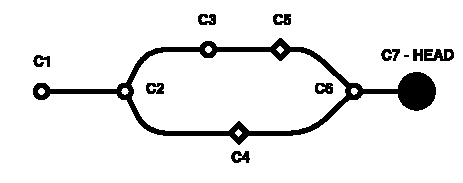
\includegraphics[width=0.5\textwidth]{cache.pdf}
    \caption{Example representation of commits history, with fix commits illustrated in a diamond shape}
    \label{fig:cache}
  \end{center}
\end{figure}


\subsection{Data Preparation}

This step is the simplest. The only task is to convert the raw JSON structure, focused on the commit, to a JSON structure, focused on the component. 7
Iterating through each file at the "\code{raw}" folder and creating a new one with the same name in the "\code{json}" folder.

The data contained in this new file will be ready for being converted to CSV and to be used for modeling or prediction.

The following columns are prepared for each component:
%
\begin{itemize}
\item \_\_changed - Was it changed?
\item \_\_filename - Component name
\item \_lines - Number of lines
\item \_bytes - File size in bytes
\item \_mostChanged - Was it the most changed file in this commit?
\item \_mostChanged25 - Was this file in top 25\% of most changed files is this commit?
\item \_mostChanged50 - Was this file in top 50\% of most changed files is this commit?
\item \_mostChanged75 - Was this file in top 75\% of most changed files is this commit?
\item changes - Number of changes made in the past
\item changes:date-weighted - Sum of the result of the time-weighted function applied to each change
\item changes:size-weighted - Sum of the number of lines added and removed in each change
\item changes:date+size-weighted - Sum of the result of the time-weighted function applied to each change multiplied for the number of lines added and removed in it
\item authors - Number of authors that changed this file
\item authorChanges::{author} - Number of changes made in the past by a specific author. E.g. authorChanges::luc@apache.org
\item authorChanges:date-weighted:{author} - Sum of the result of the time-weighted function applied to each change made by a specific author. E.g. authorChanges:date-weighted::luc@apache.org
\item authorChanges:size-weighted:{author} - Sum of the number of lines added and removed in each change made by a specific author. E.g. authorChanges:size-weighted::luc@apache.org
\item authorChanges:date+size-weighted:{author} - Sum of the result of the time-weighted function applied to each change made by a specific author multiplied for the number of lines added and removed in it. E.g. authorChanges:date+size-weighted::luc@apache.org
\end{itemize}

Being $t$ the normalized timestamp of the change, where 0 is the timestamp of the first commit and 1 of the latest, and $W = 0.5$, the time-weighted function used was the following:
%
\begin{equation}
  %\sum_{i=0}^{n}%
  \frac {1} {1 + e^{(-12 \cdot t) + (1 - W) \cdot 10 + 2}}
\end{equation}

In order to improve modeling results, we also created the columns "changes-others", "changes-others:date-weighted", "changes-others:size-weighted", "changes-others:date+size-weighted", 
"changes-fixes", "changes-fixes:date-weighted", "changes-fixes:size-weighted" and "changes-fixes:date+size-weighted" that are equal to the already existing columns starting with
"changes", but refer only to changes that were not fixes and changes that were fixes, respectively.

Plotting the results we noticed that the date influenced significantly the data related to changes, since older commits have less history behind. 
So for each, we added a normalized version by the commit.

\begin{figure}[ht]
  \begin{center}
    \leavevmode
    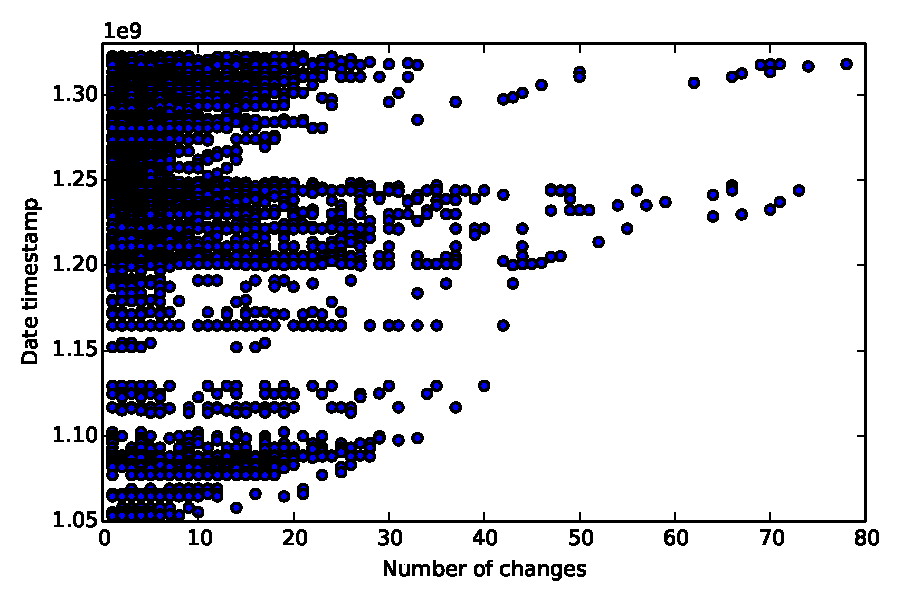
\includegraphics[width=0.75\textwidth]{date-changes_raw_math001.pdf}
    \caption{Example of the influence of the date on number of changes. (Project Math, Defect 1)}
    \label{fig:date-changes.raw}
  \end{center}
\end{figure}

\begin{figure}[ht]
  \begin{center}
    \leavevmode
    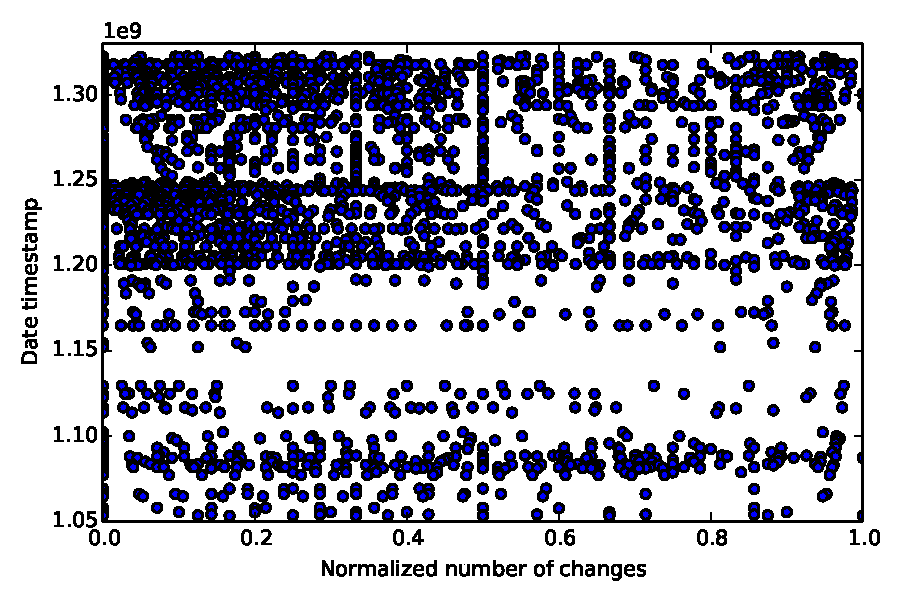
\includegraphics[width=0.75\textwidth]{date-changes_norm_math001.pdf}
    \caption{Example of the relation between the date on the normalized number of changes. (Project Math, Defect 1)}
    \label{fig:date-changes.norm}
  \end{center}
\end{figure}

\begin{lstlisting}
[
  {
    "__changed": true,
    "__date": 1364521362,
    "__filename": "src/main/java/org/apache/commons/math3/distribution/fitting/MultivariateNormalMixtureExpectationMaximization.java",
    "_lines": 441,
    "_bytes": 18211,
    "_mostChanged": false,
    "_mostChanged25": true,
    "_mostChanged50": true,
    "_mostChanged75": true,
    "changes:raw": 3,
    "changes:normalized": 0.2857142857142857,
    "changes-fixes:raw": 0,
    "changes-fixes:normalized": 0,
    "changes-others:raw": 3,
    "changes-others:normalized": 0.3333333333333333,
    "changes:date-weighted:raw": 2.979453,
    "changes:date-weighted:normalized": 0.290809968305134,
    "changes:size-weighted:raw": 481,
    "changes:size-weighted:normalized": 0.4746494066882416,
    "changes:date+size-weighted:raw": 477.701982,
    "changes:date+size-weighted:normalized": 0.4831911672918317,
    "changes-fixes:date-weighted:raw": 0,
    "changes-fixes:date-weighted:normalized": 0,
    "changes-fixes:size-weighted:raw": 0,
    "changes-fixes:size-weighted:normalized": 0,
    "changes-fixes:date+size-weighted:raw": 0,
    "changes-fixes:date+size-weighted:normalized": 0,
    "changes-others:date-weighted:raw": 2.979453,
    "changes-others:date-weighted:normalized": 0.3394176672358086,
    "changes-others:size-weighted:raw": 481,
    "changes-others:size-weighted:normalized": 0.4845814977973568,
    "changes-others:date+size-weighted:raw": 477.701982,
    "changes-others:date+size-weighted:normalized": 0.49340824785460163,
    "authors:raw": 3,
    "authors:normalized": 0.6666666666666666,
    "authorChanges::luc@apache.org:raw": 1,
    "authorChanges::luc@apache.org:normalized": 0,
    ...
    "authorChanges:date-weighted::luc@apache.org:raw": 0.993164,
    "authorChanges:date-weighted::luc@apache.org:normalized": 0.00025474141229450394,
    "authorChanges:size-weighted::luc@apache.org:raw": 33,
    "authorChanges:size-weighted::luc@apache.org:normalized": 0.5454545454545454,
    "authorChanges:date+size-weighted::luc@apache.org:raw": 32.774417,
    "authorChanges:date+size-weighted::luc@apache.org:normalized": 0.5455704368440787,
    ...
  },
  ...
]
\end{lstlisting}


The data from the multiple fix commits is then combined in a file named "history.csv" and the data from the \emph{HEAD} commit is placed at "master.csv". 
These two files will be only files required to execute the next step.


\subsection{Modeling and Prediction}

For modeling and predicting \emph{Python 3} and \emph{scikit-learn} is used.
Random Forests, Decision Trees and Naive Bayes were tried, but the former achieved significantly better results as it is presented in the Experimental Results chapter \ref{chap:exp-results}.
Neural Networks were not used since the training set is normally small.

Before training the model, the training set is randomized and balanced, first to a ratio of 5 \emph{clean} component for each \emph{buggy} component 
and then SMOTE is used to create more \emph{buggy} component entries. In order to train the model a \emph{Stratified KFold} (4 folds) is used and run 10 times, 
generating 40 different models. Performance of these 40 models is measured according to the difference of the mean defect probability of buggy test data and clean test data. 
The 15 models with the highest difference are then used to predict the defect probability of each component in the current project state and a mean is calculated.

As referred before, the results are saved directly at the repository folder.
